\documentclass[11pt, titlepage]{article}
\usepackage{beamerarticle}
\usepackage[utf8]{inputenc}
\usepackage{hyperref}
\usepackage{amssymb,amsmath}

% Page settings
\usepackage[letterpaper, margin=1in]{geometry}
\usepackage{palatino}%\usepackage{lmodern, times}
\usepackage{setspace}                           
\onehalfspacing %\doublespacing  % \singlespacing 

% Appendix
\usepackage{appendix}

% Line numbers
%\usepackage{lineno}
%\linenumbers


% Tables
\usepackage{array,booktabs,longtable,rotating}
\newenvironment{tablenotes}[1][]{
  \begin{minipage}{\textwidth}\emph{Notes:}{\footnotesize #1}
}{\end{minipage}}
\makeatletter
\def\fps@table{htbp}
\makeatother

% Graphics
\usepackage{graphicx,grffile}
\makeatletter
\def\maxwidth{\ifdim\Gin@nat@width>\linewidth\linewidth\else\Gin@nat@width\fi}
\def\maxheight{\ifdim\Gin@nat@height>\textheight\textheight\else\Gin@nat@height\fi}
\makeatother
% Scale images if necessary, so that they will not overflow the page
% margins by default, and it is still possible to overwrite the defaults
% using explicit options in \includegraphics[width, height, ...]{}
\setkeys{Gin}{width=\maxwidth,height=\maxheight,keepaspectratio}
% set default figure placement to htbp
\makeatletter
\def\fps@figure{htbp}
\makeatother

\usepackage{natbib}% plainnat
\bibliographystyle{aer}


\setlength{\emergencystretch}{3em}  % prevent overfull lines
\providecommand{\tightlist}{%
  \setlength{\itemsep}{0pt}\setlength{\parskip}{0pt}}



\institute{}
\titlegraphic{}

\usepackage{xcolor}
\newcommand\todonote[1]{\textcolor{red}{#1}}



% Subscript
\newcommand\sub[1]{_{#1}}
\newcommand\supsc[1]{^{#1}}

\title{Online Appendix: Contributing to Public Goods Inside Organizations:
Field Experimental Evidence {[}NOT FOR PUBLICATION{]}\thanks{Blasco: Harvard Institute for Quantitative Social Science, Harvard
University, 1737 Cambridge Street, Cambridge, MA 02138 (email:
\href{mailto:ablasco@fas.harvard.edu}{\nolinkurl{ablasco@fas.harvard.edu}}).
Jung: Harvard Business School, Soldiers Field, Boston, MA 02163 (email:
\href{mailto:ojung@hbs.edu}{\nolinkurl{ojung@hbs.edu}}), Lakhani:
Harvard Business School, Soldiers Field, Boston, MA 02163, and National
Bureau of Economic Research (email:
\href{mailto:k@hbs.edu}{\nolinkurl{k@hbs.edu}}). Menietti: Harvard
Institute for Quantitative Social Science, Harvard University, 1737
Cambridge Street, Cambridge, MA 02138 (email:
\href{mailto:mmenietti@fas.harvard.edu}{\nolinkurl{mmenietti@fas.harvard.edu}}).
We gratefully acknowledge the financial support of the MacArthur
Foundation (Opening Governance Network), NASA Tournament Lab, and the
Harvard Business School Division of Faculty Research and Development.
This project would not have been possible without the support of Eric
Isselbacher, Julia Jackson, Maulik Majmudar and Perry Band from the
Massachusetts General Hospital's Healthcare Transformation Lab.}}
\author{Andrea Blasco \and Olivia S. Jung \and Karim R. Lakhani \and Michael Menietti}
\date{Last updated: 13 January, 2017}

\begin{document}
\maketitle
\begin{abstract}
In this online appendix, we present a formal proof of the result of
sorting in the extended model with heterogenous costs, as discussed in
the main paper. We report additional tables and results to support the
analysis discussed in the main text. We also provide copy of the
solicitation sent, the graphics used for the headings of the website,
and the text of the `rules of the competition' page of the contest's
website.


\end{abstract}


% Todo notes
%\usepackage[textsize=tiny]{todonotes}
%\newcommand\redmarginpar[1]{\marginpar{\footnotesize{\textcolor{red}{#1}}}}
%\listoftodos[Notes]
\clearpage
\tableofcontents
\setcounter{tocdepth}{2}
\clearpage

\section{Extended model with heterogenous
costs}\label{extended-model-with-heterogenous-costs}

In this section, consider the case of two types of individuals \(j=1,2\)
forming two groups of equal size \(n_1=n_2=n\). Individuals can decide
to contribute with a single proposal or not.

When an agent of type \(j\) decides to contribute, the expected utility
is as follows.

\begin{equation}
 u_1^j = \gamma \hat Y + \delta_j + \sum_{k_j=1}^n \sum_{k_l=0}^n \Pr(Y=k_j+k_l) \frac{R}{k_j+k_l} - c_j.
\end{equation}

The utility of not contributing is as follows.

\begin{equation}
 u_0^j = \gamma (\hat Y - 1).
\end{equation}

Equating these two conditions for all individuals gives the following
mixed-strategy equilibrium condition:

\begin{equation}
\sum_{k_j=1}^n \sum_{k_l=0}^n \Pr(Y=k_j+k_l) \frac{R}{k_j+k_l} = c_j -\delta_j + \gamma
\end{equation}

for all \(j=1,2\). To examine differences in equilibrium probabilities
\(p_1^*\) and \(p_2^*\), we use the ratio between the above equilibrium
condition for individuals of type \(j=1\) and the same expression for
agents of type \(j=2\). This gives:

\begin{equation}
\frac{\sum_{k_1=1}^n \sum_{k_2=0}^n \Pr(Y=k_1+k_2) \frac{R}{k_1+k_2}}{\sum_{k_1=0}^n \sum_{k_2=1}^n \Pr(Y=k_1+k_2) \frac{R}{k_1+k_2}} = \frac{c_1 -\delta_1 + \gamma}{c_2 -\delta_2 + \gamma}.
\end{equation}

The left hand side can be rearranged as follows.

\begin{equation}
\frac{\Pr(k_2=0) \sum_{k_1=1}^n\Pr(Y=k_1)\frac{R}{k_1} +  \sigma R}{\Pr(k_1=0) \sum_{k_2=1}^n\Pr(Y=k_2)\frac{R}{k_2} +  \sigma R} 
\end{equation}

where
\(\sigma = \sum_{k_1=1}^n \sum_{k_2=1}^n \Pr(Y=k_1+k_2) \frac{1}{k_1+k_2}\).
Using \(1-p_2=\Pr(k_2=0)\) and \(1-p_1=\Pr(k_1=0)\) together with the
density of the binomial distribution, we obtain the following simpler
expression.

\begin{equation}
\frac{(1-p_2) \frac{(1- (1-p_1)^n)}{n p_1} R +  \sigma R }{(1-p_1) \frac{(1- (1-p_2)^n)}{n p_2} R +  \sigma R}  .
\end{equation}

If \(c_1 - \delta_1 > c_2 - \delta_2\), then the above expression in
equilibrium needs to be larger than one. This inequality can be
expressed as follows:

\begin{equation}
\frac{p_2 (1-p_2)}{(1- (1-p_2)^n)}  > \frac{p_1 (1-p_1)}{(1- (1-p_1)^n)}.
\end{equation}

Hence, the inequality is satisfied only if \(p_2\) is greater than
\(p_1\). This proves the last statement reported in the Section with
predictions in this paper.

\section{Additional tables and
figures}\label{additional-tables-and-figures}

In this section, we provide additional tables and figures to support the
analysis discussed in the main text.

Tables \ref{app: proposals}, \ref{app: ratings} and \ref{app: finalist}
reports the poitn estimates of the difference in the probability of
submitting proposals, rating proposals, and being selected for
implementation respectively. Figure \ref{fig: participation} shows that
the results concerning participation rates are robust to bootstrap
resampling and Holm-Bonferroni adjustments to take into account a
multiple comparison problem. Likewise Figure \ref{fig: gender robust}
shows that the results concerning gender are robust as well.

Concerning the lack of effects on the ``intensive margin,'' Figure
\ref{fig: counts} plots the distributions of the count of projects and
words per submission in each condition showing there was no clear
difference across treatments.

As discussed in the main text, there was no difference in the the
probability of rating proposals in the peer-evaluation phase. We also
fail to detect differences in the count of rated proposals per
evaluator. Here, Figure \ref{app: rating counts} plots the histogram of
the count of rated proposals in each condition, showing that the
distributions were indeed pretty similar.

\begin{table}
\centering
\caption{Difference in the probability of submitting project proposals}
\label{app: proposals}
\begin{tabular}{@{}lccccccccc}
  \\[-1.8ex]\hline \hline \\[-1.8ex]
 & Group 1 & Group 2 & p1 & p2 & n1 & n2 & Diff & SE & Z \\ 
  \hline \\[-1.86ex]
1 & PRIZE & WPLACE & 7.4 & 5.2 & 312 & 307 & 2.2 & 1.9 & 1.1 \\ 
  2 & PRIZE & PCARE & 7.4 & 4.5 & 312 & 310 & 2.9 & 1.9 & 1.5 \\ 
  3 & PRIZE & FUND & 7.4 & 2.3 & 312 & 308 & 5.1 & 1.7 & 3 \\ 
  4 & WPLACE & PCARE & 5.2 & 4.5 & 307 & 310 & 0.7 & 1.7 & 0.4 \\ 
  5 & WPLACE & FUND & 5.2 & 2.3 & 307 & 308 & 2.9 & 1.5 & 1.9 \\ 
  6 & PCARE & FUND & 4.5 & 2.3 & 310 & 308 & 2.2 & 1.5 & 1.5 \\ 
   \\[-1.8ex]\hline \hline \\[-1.8ex]
\end{tabular}
\end{table}\begin{table}
\centering
\caption{Difference in the probability of rating project proposals}
\label{app: ratings}
\begin{tabular}{@{}lccccccccc}
  \\[-1.8ex]\hline \hline \\[-1.8ex]
 & Group 1 & Group 2 & p1 & p2 & n1 & n2 & Diff & SE & Z \\ 
  \hline \\[-1.86ex]
1 & WPLACE & PCARE & 16.3 & 15.8 & 307 & 310 & 0.5 & 3 & 0.2 \\ 
  2 & WPLACE & PRIZE & 16.3 & 13.8 & 307 & 312 & 2.5 & 2.9 & 0.9 \\ 
  3 & WPLACE & FUND & 16.3 & 11.7 & 307 & 308 & 4.6 & 2.8 & 1.6 \\ 
  4 & PCARE & PRIZE & 15.8 & 13.8 & 310 & 312 & 2 & 2.8 & 0.7 \\ 
  5 & PCARE & FUND & 15.8 & 11.7 & 310 & 308 & 4.1 & 2.8 & 1.5 \\ 
  6 & PRIZE & FUND & 13.8 & 11.7 & 312 & 308 & 2.1 & 2.7 & 0.8 \\ 
   \\[-1.8ex]\hline \hline \\[-1.8ex]
\end{tabular}
\end{table}\begin{table}
\centering
\caption{Difference in the probability of submitting finalist project proposals}
\label{app: finalist}
\begin{tabular}{@{}lccccccccc}
  \\[-1.8ex]\hline \hline \\[-1.8ex]
 & Group 1 & Group 2 & p1 & p2 & n1 & n2 & Diff & SE & Z \\ 
  \hline \\[-1.86ex]
1 & PRIZE & WPLACE & 4.5 & 3.2 & 312 & 307 & 1.2 & 1.5 & 0.8 \\ 
  2 & PRIZE & PCARE & 4.5 & 2.2 & 312 & 310 & 2.2 & 1.4 & 1.5 \\ 
  3 & PRIZE & FUND & 4.5 & 0.6 & 312 & 308 & 3.8 & 1.3 & 3 \\ 
  4 & WPLACE & PCARE & 3.2 & 2.2 & 307 & 310 & 1 & 1.3 & 0.8 \\ 
  5 & WPLACE & FUND & 3.2 & 0.6 & 307 & 308 & 2.6 & 1.1 & 2.3 \\ 
  6 & PCARE & FUND & 2.2 & 0.6 & 310 & 308 & 1.6 & 1 & 1.7 \\ 
   \\[-1.8ex]\hline \hline \\[-1.8ex]
\end{tabular}
\end{table}

\begin{figure} 
  \centering
  \caption{Pairwise comparisons of the percentage of employees submitting a project proposal in the different treatments with Holm-Bonferroni method and bootstrap resampling}
  \label{fig: participation}
  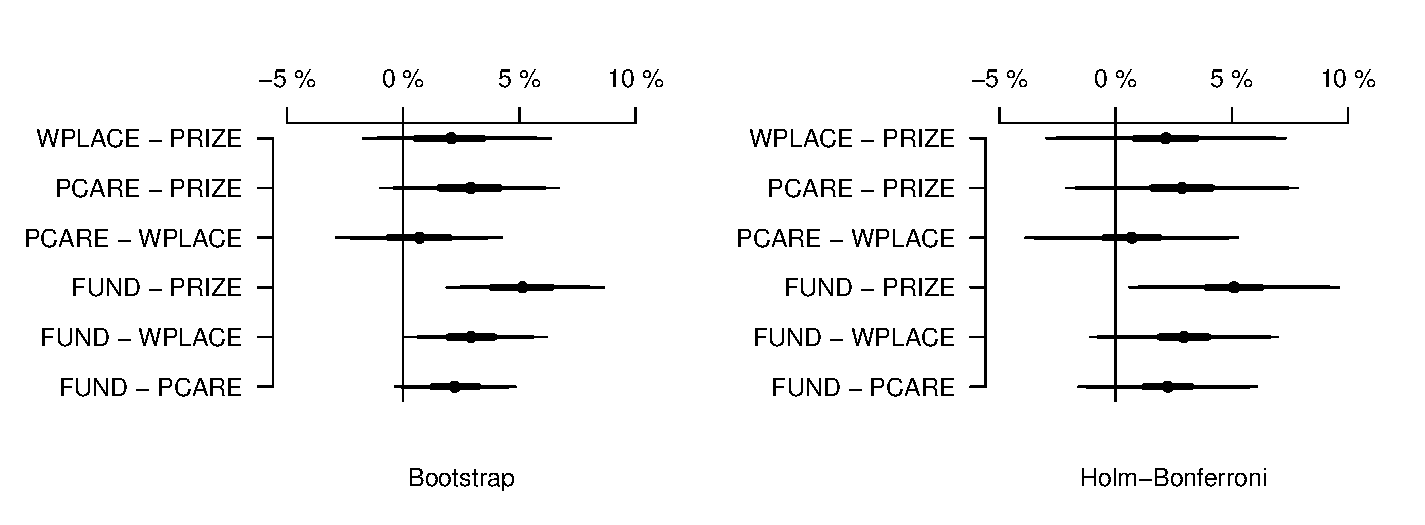
\includegraphics{Figures/pairwise-robust-1.pdf}
\end{figure}

\begin{figure} 
  \centering
  \caption{Difference in the probability of submitting between men and women with Holm-Bonferroni method and bootstrap resampling}
  \label{fig: gender robust}
  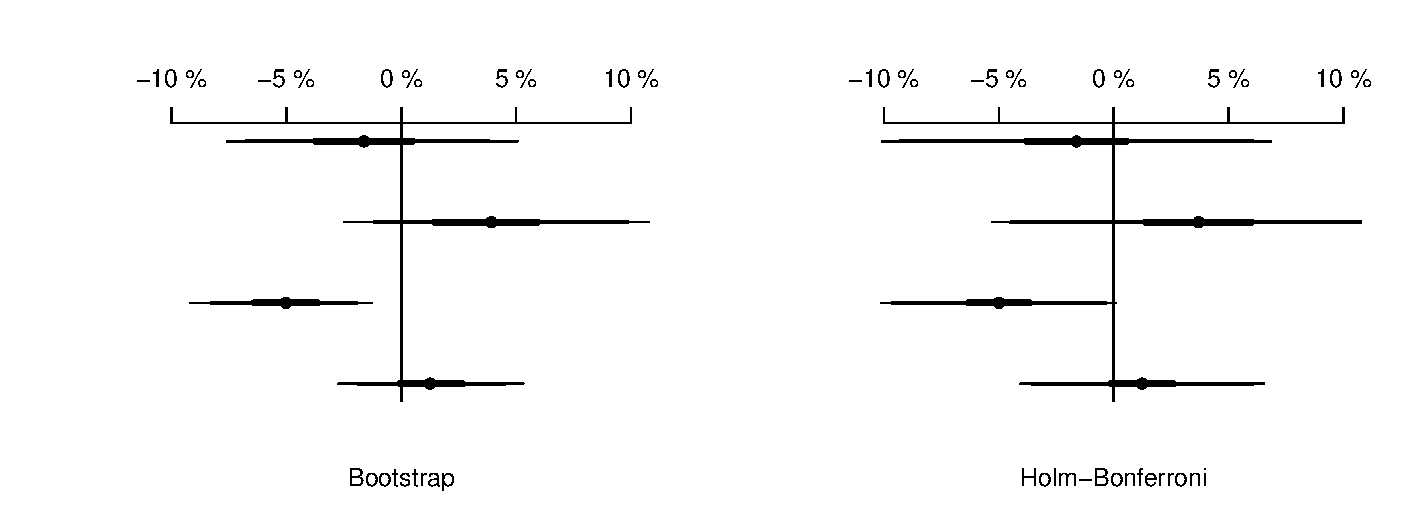
\includegraphics{Figures/gender-robust-1.pdf}
\end{figure}

\begin{figure} 
  \centering
  \caption{Count of projects (left panel) and words (right panel) per submission by treatments}
  \label{fig: counts}
  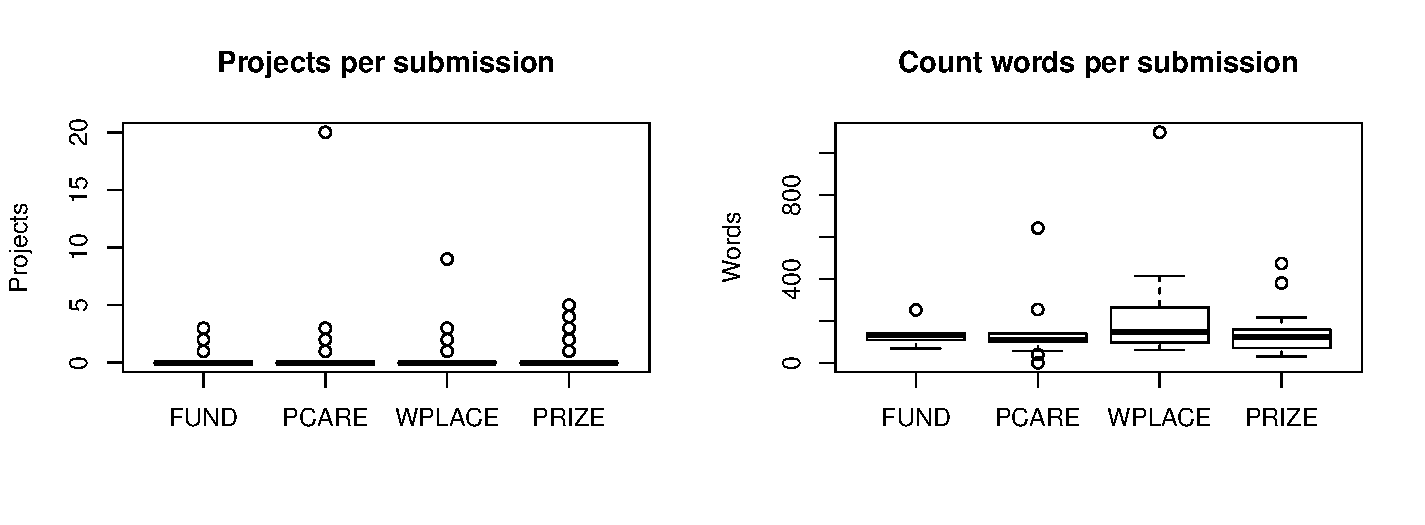
\includegraphics{Figures/counts-1.pdf}
\end{figure}

\begin{figure}
\centering
\caption{Count of the rated project proposals per evaluator}
\label{app: rating counts}
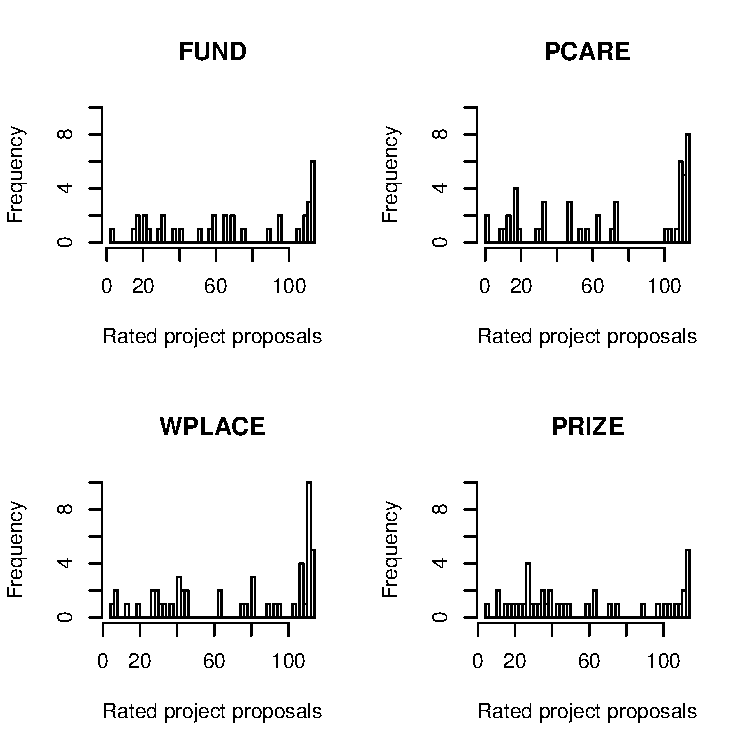
\includegraphics{Figures/plot-ratings-appendix-1.pdf}
\end{figure}

\section{Solicitation and website}\label{solicitation-and-website}

In Section \ref{solicitation-and-graphics}, Figure
\ref{app: solicitation} shows copy of the solicitation sent via email
and Figure \ref{app: graphics} shows the graphics automatically matching
the treatment of the employee signing in to the contest's website. In
Section \ref{rules-of-the-competition}, we report the text displayed in
the ``Rules of the Competition'' section of the contest's website.

\subsection{Solicitation and Graphics}\label{solicitation-and-graphics}

\begin{figure}
\centering
\caption{Copy of the solicitation sent via email to the employees in our subject pool}
\label{app: solicitation}
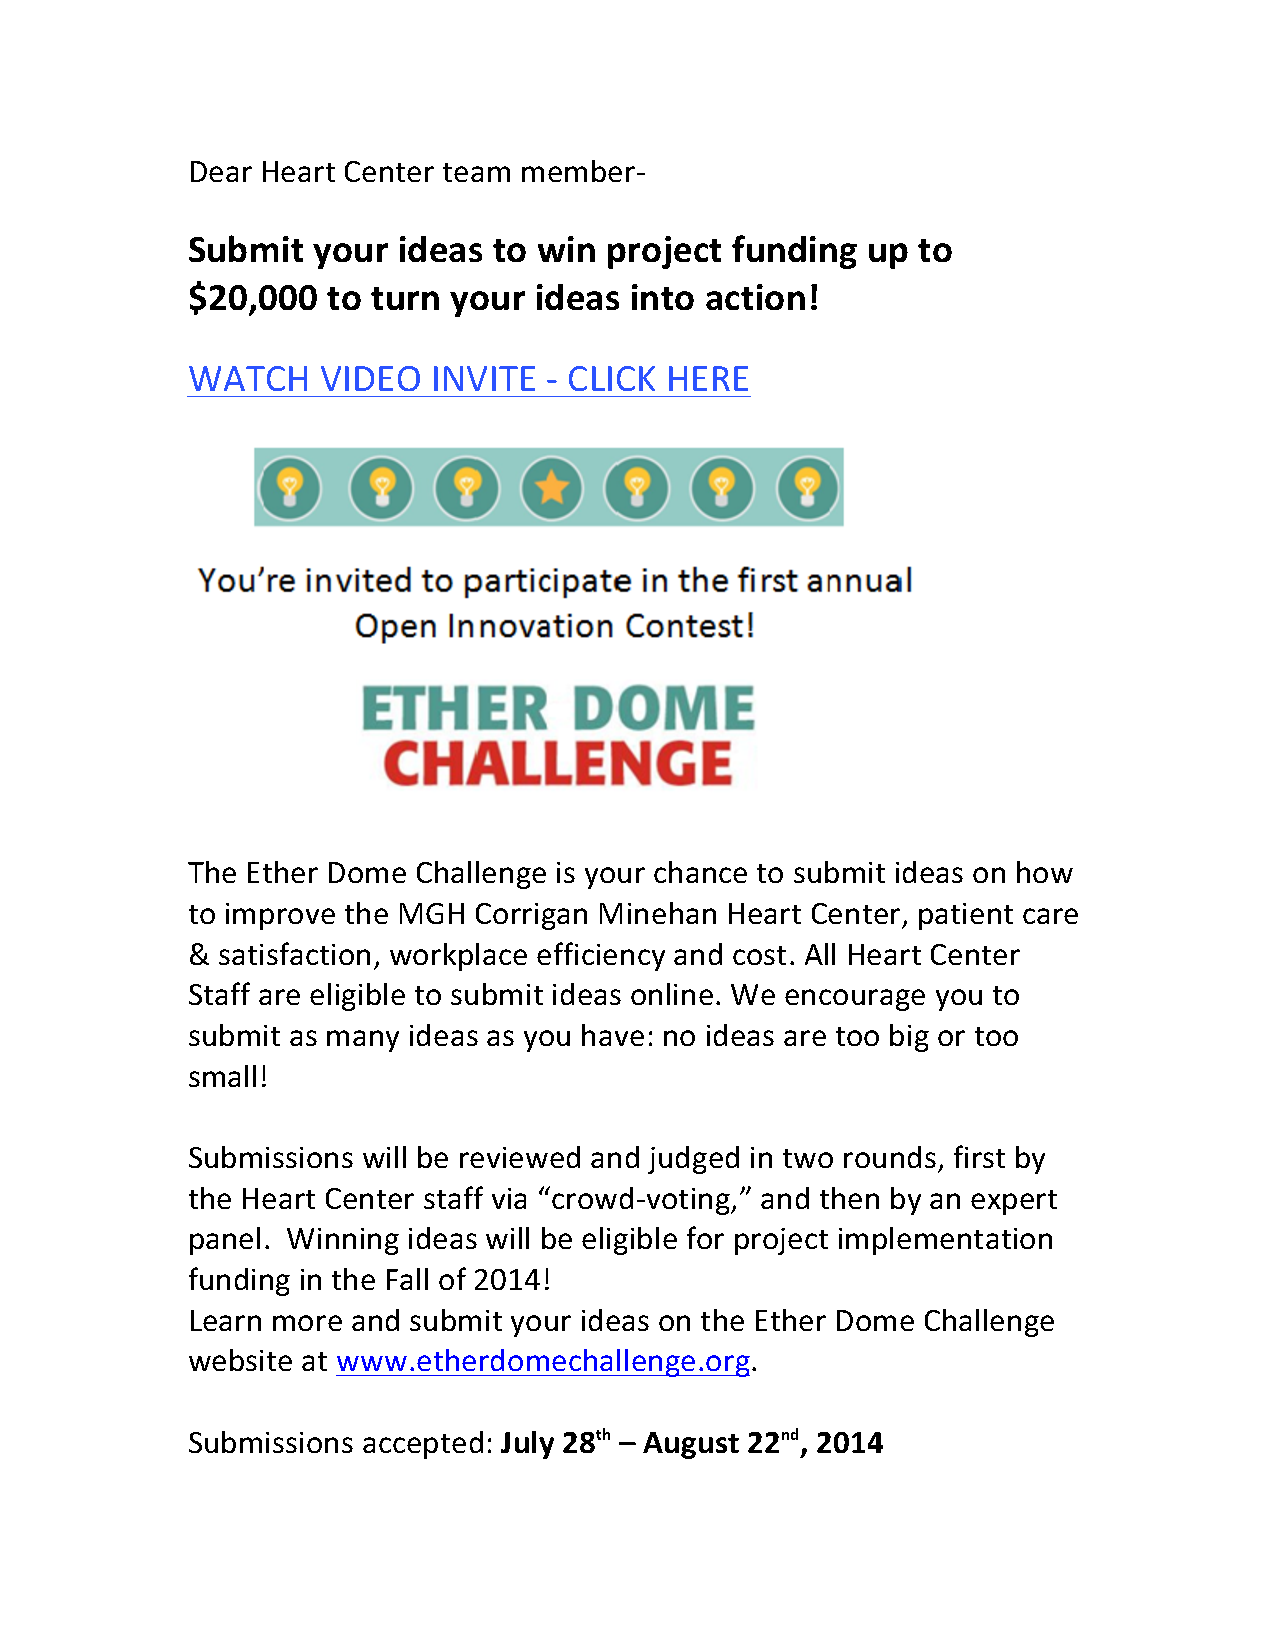
\includegraphics[width=\textwidth]{Images/solicitationEmail.pdf}
\end{figure}

\begin{figure}
\centering
\caption{Graphics matching the treatment of the employee signing in to the contest's website}
\label{app: graphics}
\begin{tabular}{cc}

\includegraphics[width=2in, height=1.5in]{Images/priming/funding.png} & 

\includegraphics[width=2in, height=1.5in]{Images/priming/money.png} \\
FUND & PRIZE \\

\includegraphics[width=2in, height=1.5in]{Images/priming/patientcare.png} & 
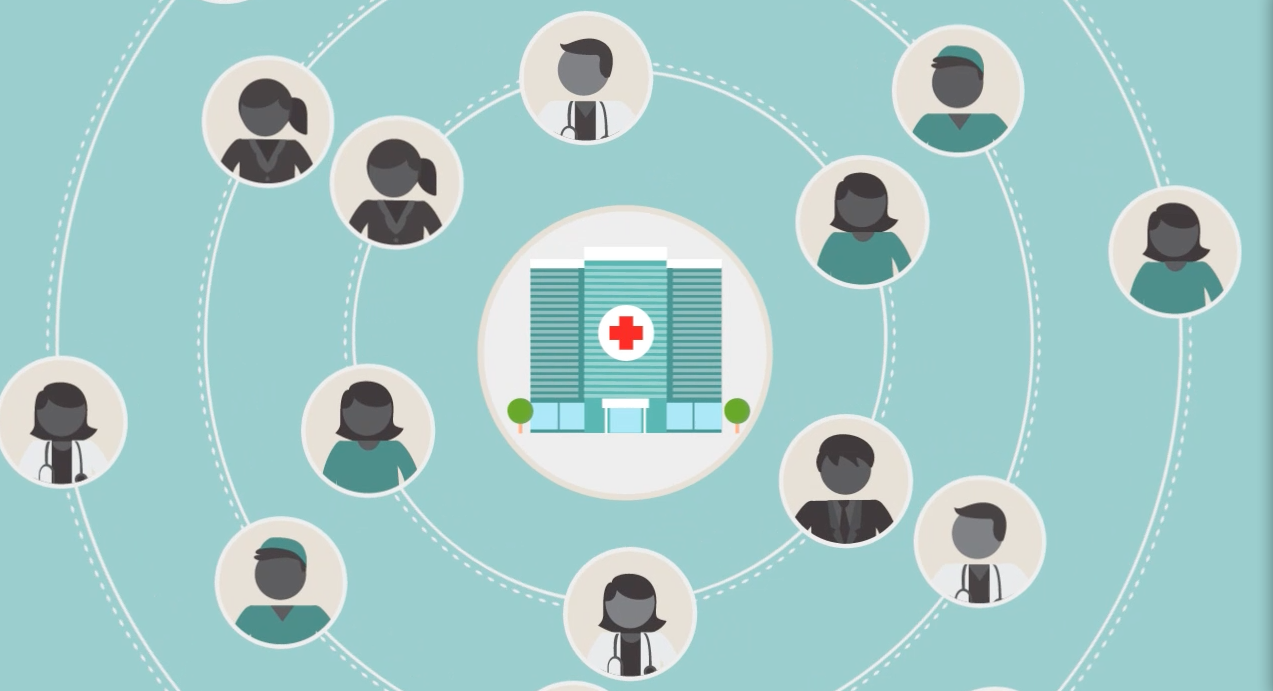
\includegraphics[width=2in, height=1.5in]{Images/priming/workplace.png} \\
PCARE & WPLACE
\end{tabular}
\end{figure}

\clearpage

\subsection{Rules of the competition}\label{rules-of-the-competition}

\begin{itemize}
\item
  The Ether Dome Challenge is an ideas competition to improve the Heart
  Center workplace, patient care, patient satisfaction, workplace
  efficiency and cost.
\item
  If you've noticed something about patient experience, employee
  satisfaction, workplace efficiency, or anything that could be
  improved; if you've had an inspiration about a new way to safeguard
  health; or if you simply have a cost-saving idea, then now is the time
  to share your idea. We would like to encourage all members of the
  Heart Center to participate in this initiative. We encourage you to
  submit as many ideas as you have: no ideas are too big or too small!
  You never know\ldots{} your idea could be the next big thing!
\end{itemize}

\emph{Timeline}

\begin{itemize}
\tightlist
\item
  Ideation Contest Launch
\item
  Idea Submission Closes
\item
  Crowd-Voting on Submitted Ideas
\item
  Top 3 Crowd Voting Winners Announced (winners will receive iPads) \&
  Final Round Idea Selections Announced
\item
  Final Round Idea ``Brainstorming'' Support Sessions \& Team
  Submissions Accepted
\item
  Final Round Submissions Due
\item
  Judging Panel Review of Final Round Submissions
\item
  Ether Dome Challenge Final Award Event - Grant Winners Announced!
\end{itemize}

\emph{Logistics of Idea Submissions}

\begin{itemize}
\tightlist
\item
  All Heart Center Staff (physicians, nurses, administrators, etc.) are
  eligible to submit Ideas.
\item
  Ideas should be submitted electronically via this site. Please click
  the ``Submit Your Ideas'' button at the top of the page, to enter the
  Challenge.
\item
  Submit as many ideas as you'd like!
\end{itemize}

\emph{To promote all kinds of ideas\ldots{} even the zanny ones!}

\begin{itemize}
\tightlist
\item
  All ideas submitted during the challenge will be posted on this
  website to be voted on by all Heart Center staff. The best ideas will
  be awarded a prize. To keep voting fair, ideas will be anonymously
  posted to the voting site. If your idea wins, you will be able to
  choose whether or not you'd like recognition for the idea. To ensure
  everyone feels free to submit all types of creative ideas - no matter
  how disruptive - all ideas will remain anonymous and shared only with
  the Harvard Business School study designers and the MGH Healthcare
  Transformation Lab staff. Individual information/ideas will not be
  shared with your managers/division heads, unless you elect for it to
  be shared publicly after the voting period. De-identified idea
  submissions will be shared with all levels of hospital administration
  deemed appropriate by the Healthcare Transformation Lab staff.
\end{itemize}

\emph{Areas of focus - but don't limit your thinking!}

\begin{itemize}
\tightlist
\item
  Areas of focus for the Ether Dome Challenge include, but are not
  limited to: New models of care delivery; Enhancing the patient
  experience; Improving the MGH workplace, Improving efficiency, quality
  and safety; Lowering the cost of care
\end{itemize}

\bibliography{/Users/andrea/Papers/library.bib}

\end{document}